\documentclass{article}
%Packages
\usepackage{tikz}
\usetikzlibrary{shapes,arrows, positioning}


\begin{document}

\section{How to Draw Rhomboid in LaTex}
  

%Example1
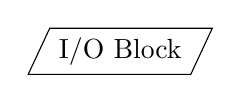
\begin{tikzpicture}
	\node[draw,
	     trapezium,
		 trapezium left angle = 65,
		 trapezium right angle = 115,
		 trapezium stretches]{I/O Block}; % since this is trapezium so draw trapezium, and left hand angle is 65 degree and right hand side angle is 115 degree,
% You can use the stretch mark for the fixed fitting.

\end{tikzpicture}

%Example 2
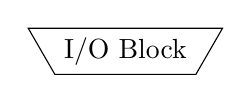
\begin{tikzpicture}
	\node[draw,
	     trapezium,
		 trapezium left angle = 120,
		 trapezium right angle = 120,
		 trapezium stretches]{I/O Block};
\end{tikzpicture}



\end{document}


